\chapter{Requisiti Software}
\raggedright{\section{Modellazione casi d'uso richiesti}}
All'interno della nostra applicazione rimodernizzata, da qui in avanti chiamata \textit{Alexandria}, abbiamo individuato 6 casi d'uso: un caso d'uso relativo all'autenticazione, un caso d'uso relativo alla ricerca dei riferimenti e autori, un caso d'uso relativo alla creazione dei riferimenti, un caso d'uso relativo alla creazione delle categorie, un caso d'uso relativo alla visualizzazione e creazione modifica dei propri riferimenti e infine caso d'uso relativo alle impostazioni utente.
         \begin{center}
     \hspace{-1cm}
            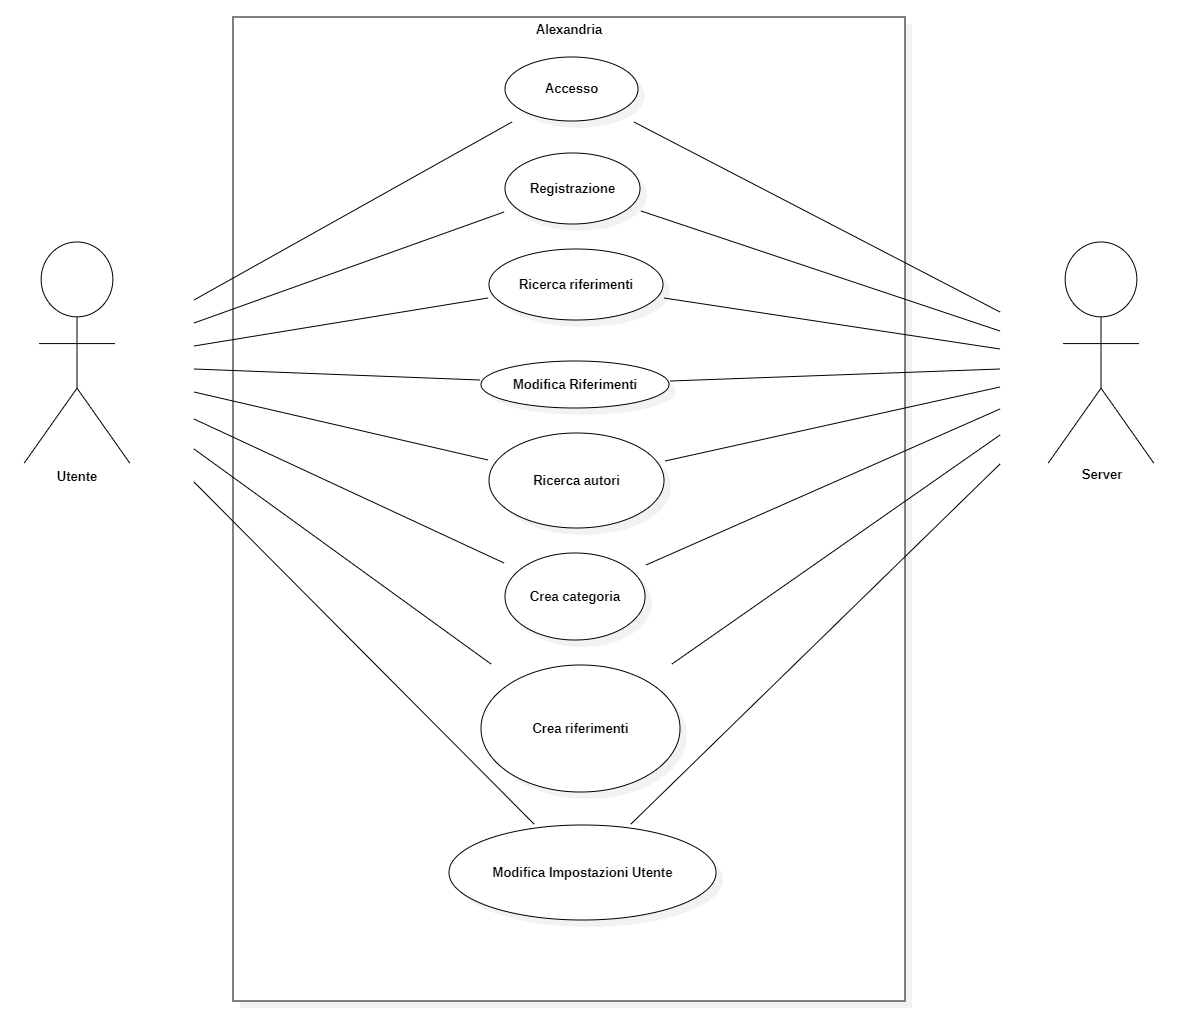
\includegraphics[width=.90\textwidth]{Immagini/Alexandria/useCase.png} 
        \end{center}


\raggedright{\section{Individuazione target degli utenti}}
Il bacino d'utenza principale saranno gli utenti che intendono gestire e visualizzare sia i propri riferimenti bibliografici, sia quelli degli altri utenti presenti nel sistema. Altri utenti che potranno essere interessati a utilizzare l'applicativo sono gli autori stessi dei riferimenti bibliografici, le case editrici che gestiscono le varie edizioni dei riferimenti. 

\raggedright{\section{4 casi d'uso in particolare}}
\raggedright{\subsection{Caso d'uso: Ricerca}}
\raggedright{\subsection{Caso d'uso: Creazione Riferimento}}
\raggedright{\subsection{Caso d'uso: Ricerca}}
\raggedright{\subsection{Caso d'uso: Modifica propri Riferimenti}}
\raggedright{\subsection{Caso d'uso: Crea Categoria}}






\raggedright{\section{MockUp Interfaccia grafica}}

\raggedright{\section{Valutazione dell'usabilità}}

\raggedright{\section{Glossario}}

\raggedright{\section{Classi, oggetti e relazioni d'analisi}}

\raggedright{\section{Diagrammi di Sequenza}}

\raggedright{\section{Prototipazione funzionale}}









